% Nallino, Part I p. 253: Schiaparelli's figure of the epicycle of Mercury, redrawn from the print: the arc AB of
% the orbit of the Sun, the epicycle CD about I touching it at C, the line from C through I and D to the Earth T,
% and the bold italic letters. Measured on the scan (_intake/latin/tools/fig253).
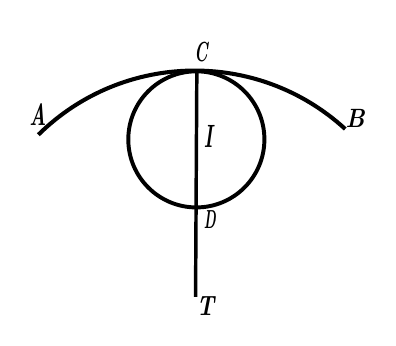
\begin{tikzpicture}[x=0.9964pt,y=-0.9964pt,line cap=butt,every node/.style={font=\fontsize{11}{11}\bfseries\itshape\selectfont,inner sep=0pt}]
\useasboundingbox (0,0) rectangle (123.20,105.20);
\draw[line width=1.42pt] (61.17,40.51) circle[radius=24.68];  % the epicycle CD about I
\draw[line width=1.25pt] (61.35,15.52) -- (60.88,97.62);  % the line from C through I and D to T
\draw[line width=1.47pt] (3.86,38.84) arc[start angle=-134.62,end angle=-47.54,radius=80.80];
\node at (62.90,8.82) {\normalfont\fontsize{11}{11}\bfseries\itshape\selectfont \resizebox{4.83pt}{6.83pt}{C}};
\node at (3.64,31.54) {\normalfont\fontsize{11}{11}\bfseries\itshape\selectfont \resizebox{6.11pt}{7.63pt}{A}};
\node at (118.78,33.00) {\normalfont\fontsize{11}{11}\bfseries\itshape\selectfont \resizebox{6.90pt}{6.56pt}{B}};
\node at (65.53,39.36) {\normalfont\fontsize{11}{11}\bfseries\itshape\selectfont \resizebox{3.17pt}{7.99pt}{I}};
\node at (66.04,69.44) {\normalfont\fontsize{11}{11}\bfseries\itshape\selectfont \resizebox{4.34pt}{6.46pt}{D}};
\node at (64.49,100.76) {\normalfont\fontsize{11}{11}\bfseries\itshape\selectfont \resizebox{6.36pt}{6.92pt}{T}};
\end{tikzpicture}
